\section*{Counter Sheets}
\addcontentsline{toc}{section}{Counter Sheets}

The complete 200-counter sheet is reconstructed below in its original
20-by-10 arrangement. Every die-cut position is shown, including unused blank
faces. Counter colors have been restored from the surviving printed sheet.

\begin{center}
  {\sffamily\bfseries\large Front\par}
  \vspace{3pt}
  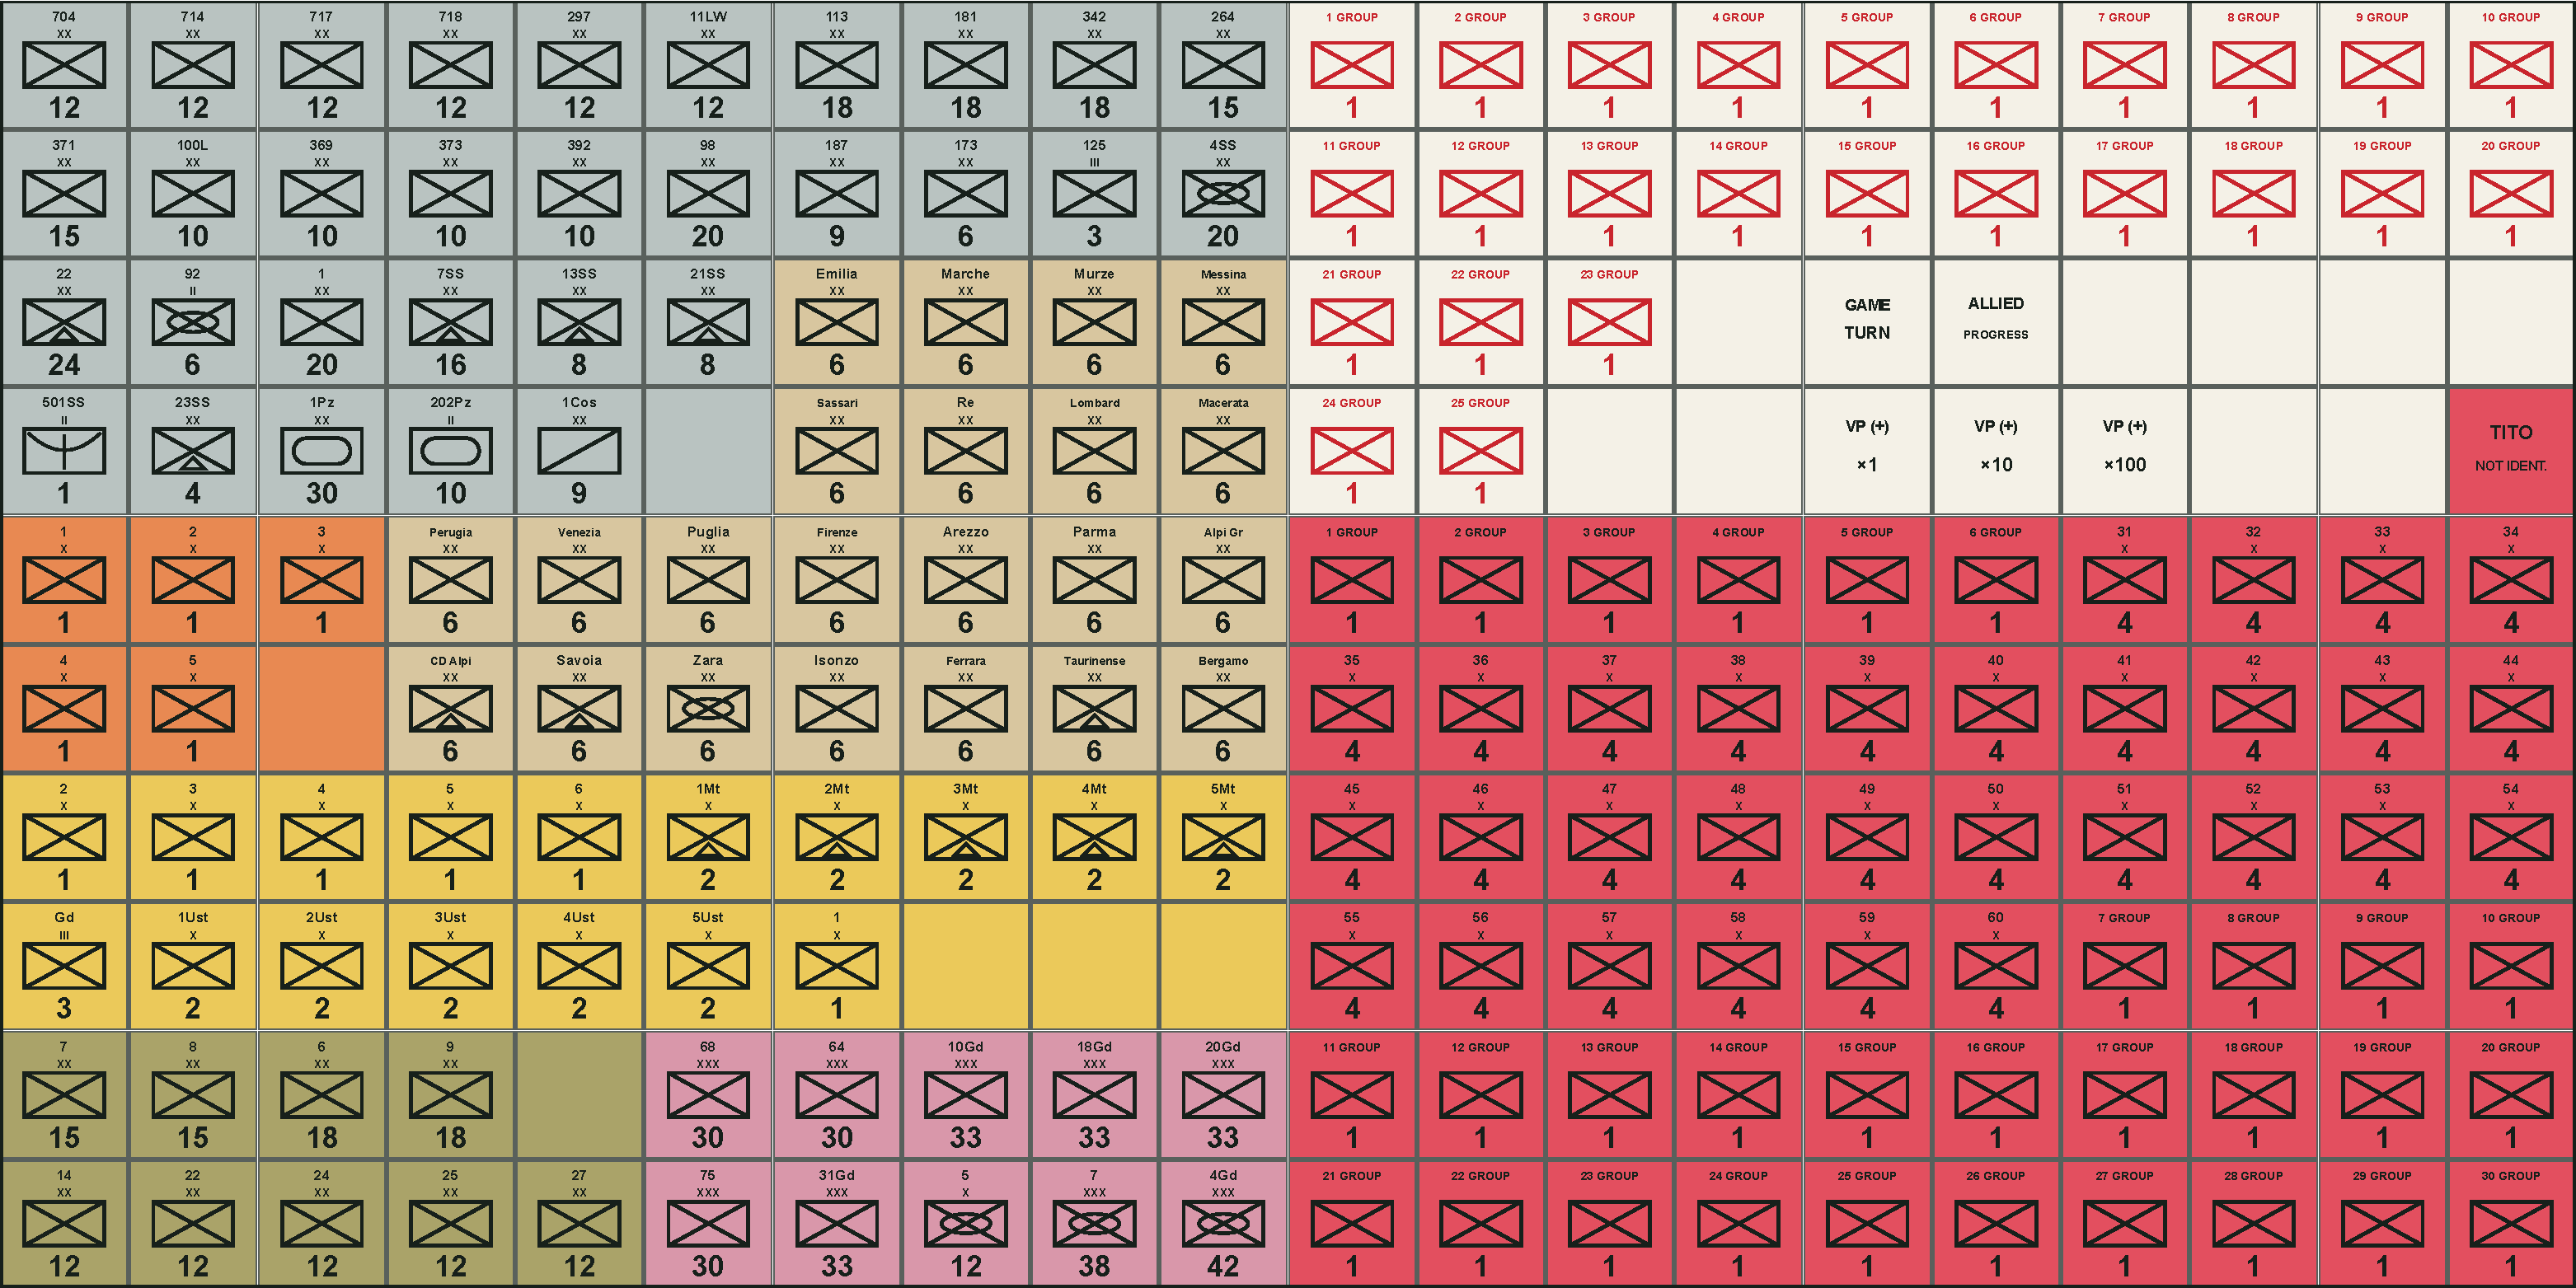
\includegraphics[width=\textwidth]{figures/counter-sheet-front.pdf}

  \vspace{9pt}
  {\sffamily\bfseries\large Back\par}
  \vspace{3pt}
  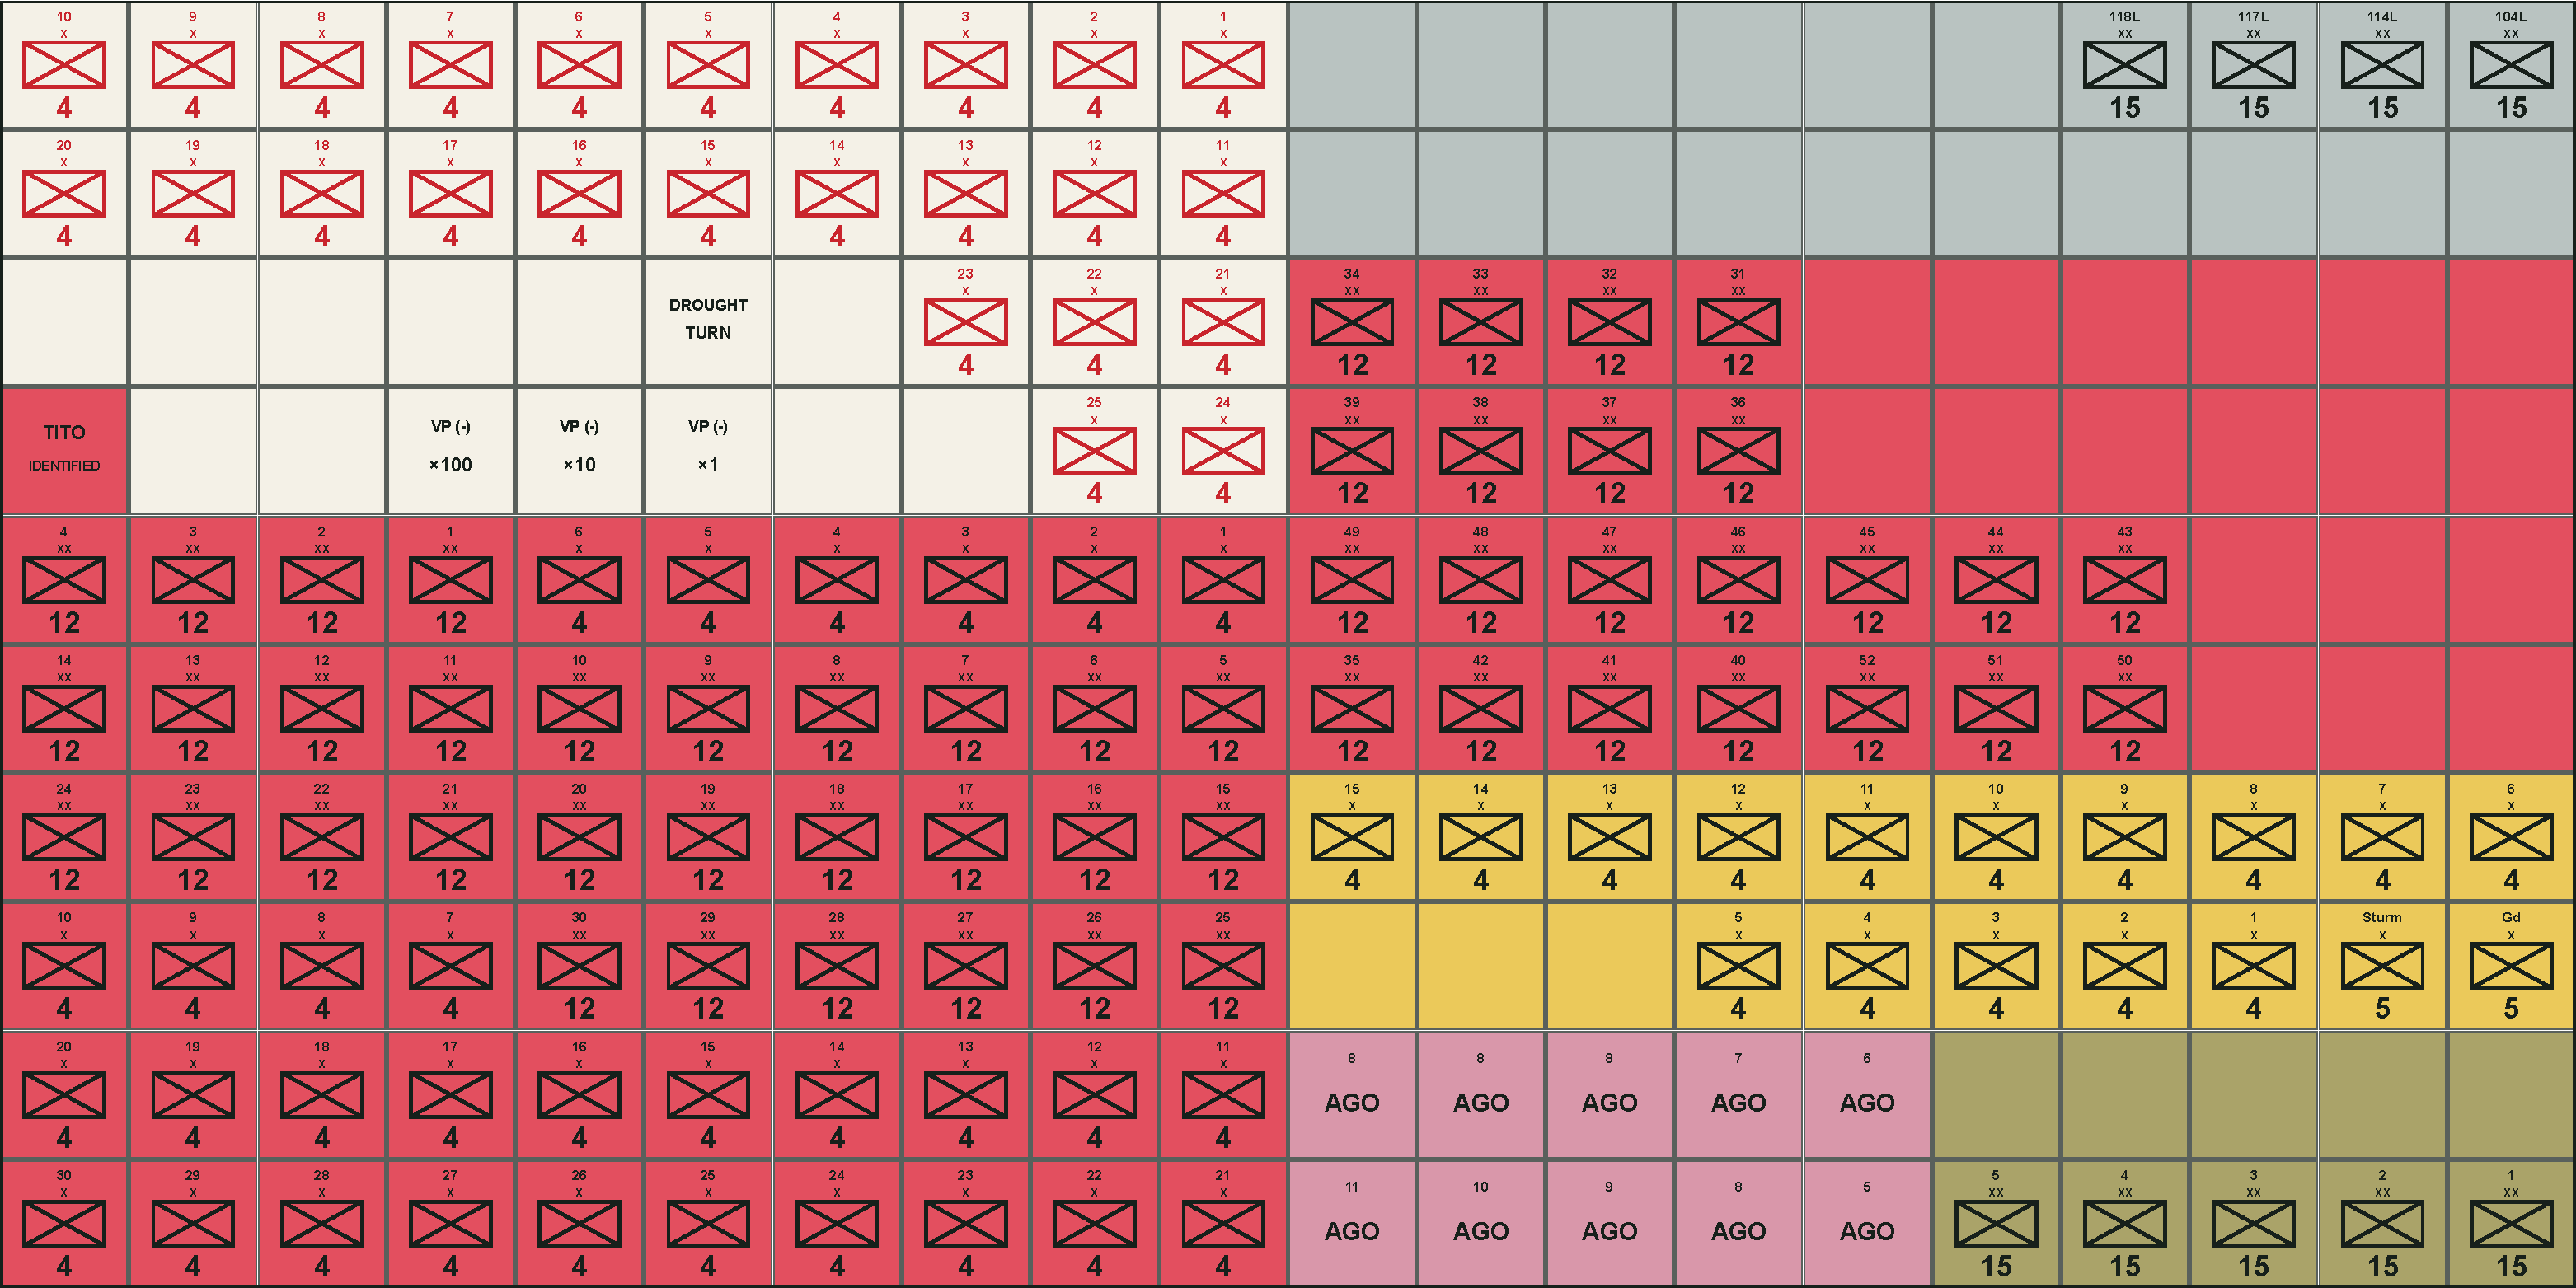
\includegraphics[width=\textwidth]{figures/counter-sheet-back.pdf}
\end{center}

\vfill
{\footnotesize\itshape Unit designations, strengths, quantities, and reverse
faces follow the counter manifest supplied with the original game.}
